\section{Introduction to Plutus Language} \label{sec:Languages}

\begin{quote}
Plutus is the native smart contract language for Cardano. It is a Turing-complete language written in Haskell, and Plutus smart contracts are effectively Haskell programs. By using Plutus, you can be confident in the correct execution of your smart contracts. It draws from modern language research to provide a safe, full-stack programming environment based on Haskell, the leading purely functional programming language.
\end{quote}


The Plutus Playground has been recently updated, providing a platform for developing smart contract applications using Haskell. At its core, the Plutus Platform enables developers to write smart contracts in Haskell, a high-level, robust programming language. This setup ensures that users can rely on well-established tooling and libraries without needing to learn a new, proprietary language.

\subsection{Plutus Tx Compiler}
The key technology that facilitates this is Plutus Tx, which acts as a compiler from Haskell to Plutus Core, the language executed on the Cardano blockchain. Provided as a GHC (Glasgow Haskell Compiler) plug-in, Plutus Tx compiles Haskell code into executable files for users' computers and Plutus Core for blockchain execution.

\subsection{Handling Haskell’s Complexity}
Haskell, known for its complexity and numerous sophisticated extensions, is simplified through the design of GHC. GHC Core, a straightforward representation of Haskell programs, allows the complex surface language to be desugared after initial type checking. This process lets Plutus Tx operate on GHC Core, benefiting from the extensive Haskell language support.

\begin{quote}
``Fortunately, the design of GHC, the primary Haskell compiler, makes this possible. GHC has a very simple representation of Haskell programs called GHC Core. After the initial typechecking phase, all of the complex surface language is desugared away into GHC Core, and the rest of the pipeline doesn’t need to know about it. This works for us too: we can operate on GHC Core, and get support for the much larger Haskell surface language for free.''
\end{quote}

While Haskell's type system is complex, Plutus Tx leverages a subset of it, sufficient for blockchain needs. However, not all Haskell features are supported, particularly those irrelevant or difficult to implement on the blockchain. The compiler provides helpful errors when unsupported features are used.

\subsection{Compilation Pipeline}
The compilation process involves multiple stages, utilizing intermediate languages to break down the tasks. The pipeline includes:

\begin{enumerate}
    \item GHC: Haskell to GHC Core
    \item Plutus Tx compiler: GHC Core to Plutus IR
    \item Plutus IR compiler: Plutus IR to Typed Plutus Core
    \item Type eraser: Typed Plutus Core to Untyped Plutus Core
\end{enumerate}

Plutus IR, closely aligned with GHC Core, reduces the logic within the plug-in and allows for independent testing of subsequent stages.

\subsection{Integration with GHC}
Plutus Tx integrates into the GHC compilation pipeline through GHC plug-ins, which modify the program during compilation. This integration enables the Plutus Tx compiler to produce Plutus Core, embedded back into the Haskell program as an opaque byte string ready for blockchain transactions.

\begin{quote}
``Because we are able to modify the program GHC is compiling, we have an obvious place to put the output of the Plutus Tx compiler, back into the main Haskell program! That’s the right place for it, because the rest of the Haskell program is responsible for submitting transactions containing Plutus Core scripts. But from the point of view of the rest of the program, Plutus Core is opaque, so we can get away with just providing it as a blob of bytes ready to go into a transaction.''
\end{quote}

\subsection{Runtime Considerations}
Dynamic elements of smart contracts, such as participant details or transaction amounts, require runtime variability. This is addressed using type classes like \texttt{Typeable} and \texttt{Lift}, which facilitate turning Haskell types and values into Plutus Core representations.

\subsection{References}
For more detailed information, visit the Plutus Playground and follow the development on \href{https://github.com/input-output-hk/plutus}{GitHub}.


\subsection{Setting Up the Environment}

To build the Plutus development environment on an Ubuntu 20.04 VM, follow these steps:

\subsection{Installing Haskell and Components}

\begin{enumerate}
    \item \textbf{Create and start a VM:}
    \begin{itemize}
        \item Create a VM with at least 8 GB of RAM and 100 GB of storage, and select Ubuntu 64-bit.
        \item Install Ubuntu 20.04 on the VM.
    \end{itemize}
    
    \item \textbf{Update and upgrade the system:}
    \begin{verbatim}
    sudo apt update
    sudo apt upgrade -y
    \end{verbatim}
    
    \item \textbf{Install Haskell:}
    \begin{verbatim}
    sudo apt-get install haskell-platform
    \end{verbatim}
    
    \item \textbf{Install \texttt{ghcup} and required dependencies:}
    \begin{verbatim}
    sudo apt install curl
    sudo apt install build-essential curl libffi-dev libffi6 libgmp-dev 
    libgmp10 libncurses-dev libncurses5 libtinfo5 libsodium-dev
    curl --proto '=https' --tlsv1.2 -sSf https://get-ghcup.haskell.org | sh
    \end{verbatim}
    \textit{Restart your terminal.}
    
    Check the Haskell version:
    \begin{verbatim}
    ghc --version
    cabal --version
    \end{verbatim}
    
    \item \textbf{Clone the Plutus repositories:}
    \begin{verbatim}
    sudo apt install git
    mkdir cardano
    cd cardano
    git clone https://github.com/input-output-hk/plutus
    git clone https://github.com/input-output-hk/plutus-pioneer-program
    \end{verbatim}
    \textit{Run \texttt{cabal update} and \texttt{cabal build} each time you start on a different section of the homework.}
\end{enumerate}

\subsection{Installing \texttt{nix-shell} and Plutus Binaries}

\begin{enumerate}
    \item \textbf{Install the cache:}
    \begin{verbatim}
    sudo mkdir /etc/nix
    \end{verbatim}
    Create a file named \texttt{nix.conf} in \texttt{/etc/nix/} with the following content:
    \begin{verbatim}
    substituters        = https://hydra.iohk.io https://iohk.cachix.org 
    trusted-public-keys = hydra.iohk.io:f/Ea+s+dFdN+3Y/
    G+FDgSq+a5NEWhJGzdjvKNGv0/EQ=iohk.cachix.org-1:
    DpRUyj7h7V830dp/i6Nti+NEO2/nhblbov/8MW7Rqoo= 
     cache.nixos.org-1:6NCHdD59X431o0gWypbMrAURkbJ16ZPMQFGspcDShjY=
    \end{verbatim}
    
    \item \textbf{Install \texttt{nix}:}
    \begin{verbatim}
    curl -L https://nixos.org/nix/install | sh
    \end{verbatim}
    After installation, set up the environment variables as instructed. Typically, this involves running:
    \begin{verbatim}
    . /home/(user)/.nix-profile/etc/profile.d/nix.sh
    \end{verbatim}
    You may need to add \texttt{~/.nix-profile/bin} to your \texttt{/etc/environment} file and restart the computer.
    
    \item \textbf{Build Plutus with \texttt{nix-shell}:}
    \begin{verbatim}
    cd ~/cardano/plutus
    git checkout 3746610e53654a1167aeb4c6294c6096d16b0502
    nix build -f default.nix 
    plutus.haskell.packages.plutus-core.components.library
    \end{verbatim}
    \textit{This process may take a while and may produce a warning about dumping a very large path.}
    
    The first run of \texttt{nix-shell} will also take some time. The first video in the course will guide you through starting the Plutus Playground server and application.
\end{enumerate}





\subsection{Writing a Simple Smart Contract in Plutus Tx}

Here is a simple example of a smart contract in Plutus Tx. This contract verifies that the number passed in the redeemer is 42.


\definecolor{codegray}{rgb}{0.5,0.5,0.5}
\definecolor{codepurple}{rgb}{0.58,0,0.82}
\definecolor{backcolour}{rgb}{0.95,0.95,0.92}

\lstdefinestyle{mystyle}{
    backgroundcolor=\color{backcolour},   
    commentstyle=\color{codegray},
    keywordstyle=\color{magenta},
    numberstyle=\tiny\color{codegray},
    stringstyle=\color{codepurple},
    basicstyle=\ttfamily\footnotesize,
    breakatwhitespace=false,         
    breaklines=true,                 
    captionpos=b,                    
    keepspaces=true,                 
    numbers=left,                    
    numbersep=5pt,                  
    showspaces=false,                
    showstringspaces=false,
    showtabs=false,                  
    tabsize=2
}

\lstset{style=mystyle}

\lstdefinelanguage{Haskell}{
    keywords={module, import, qualified, as, data, type, where, if, then, else, otherwise},
    keywordstyle=\color{blue}\bfseries,
    ndkeywords={},
    ndkeywordstyle=\color{orange}\bfseries,
    identifierstyle=\color{black},
    sensitive=true,
    comment=[l]{--},
    morecomment=[s]{/*}{*/},
    commentstyle=\color{codegray}\ttfamily,
    stringstyle=\color{codepurple}\ttfamily,
    morestring=[b]',
    morestring=[b]"
}

% Set listing style
\lstset{
    basicstyle=\ttfamily\small,
    commentstyle=\color{codegray},
    stringstyle=\color{codepurple},
    keywordstyle=\color{blue},
    showstringspaces=false,
    tabsize=4,
    language=Haskell,
    breaklines=true,
    frame=single,
    captionpos=b
}

\lstinputlisting[]{sections/solutions/fortytwo.hs}


This contract's only function is to verify that the redeemer is 42. It generates a .plutus file, which is used to generate the address and to unlock the UTXOs in the contract.

\subsection{Additional Resources}

For readers seeking more detailed information on how to code with Plutus Tx, the following resources are highly recommended:

\begin{itemize}
    \item The \textbf{Plutus Pioneer Program documentation} offers an extensive guide on using the Plutus Playground and coding Plutus contracts. You can access the documentation at \url{https://plutus-pioneer-program.readthedocs.io/en/latest/pioneer/week1.html#to-the-playground}.
    
    \item A series of instructional \textbf{YouTube videos} is available, providing a practical overview of the Plutus Playground. You can find the playlist at \url{https://www.youtube.com/playlist?list=PLNEK_Ejlx3x3xFHJJKdyfo9eB0Iw-OQDd}.
\end{itemize}

This eBook will focus more on the latest languages and developments for Cardano smart contracts, offering a contemporary perspective on the evolving ecosystem.


\section{Exploring Helios Language} \label{sec:Languages}


The Helios language is a functional programming language with a syntax that is notably similar to C. It features a straightforward curly braces syntax and is inspired by languages like Go and Rust. Helios aims to balance simplicity and safety in the development of decentralized applications (dApps) on the Cardano blockchain.

\subsection{Tenets of Helios}

\begin{itemize}
    \item \textbf{Readability Over Writeability:} The language emphasizes code readability, ensuring that code is easy to understand and maintain.
    \item \textbf{Easily Auditable:} Helios is designed to be easily auditable, allowing developers and auditors to quickly spot potential malicious code.
    \item \textbf{Opinionated:} The language provides a single, clear way to accomplish tasks, reducing ambiguity and complexity in code development.
\end{itemize}

\subsection{Helios as a JavaScript/TypeScript SDK}

Helios serves as a JavaScript/TypeScript SDK for the Cardano blockchain, encompassing everything needed to build dApps. This includes a simple smart contract language tailored for the Cardano ecosystem.

\subsection{Setup of the Helios Library}

The Helios library is platform agnostic and supports various methods for integration:

\begin{itemize}
    \item \textbf{Webpage Script Tag:}
    \begin{verbatim}
    <script src="https://helios.hyperion-bt.org/<version>/helios.js" 
    type="module" crossorigin></script>
    \end{verbatim}
    
    \item \textbf{Module with CDN URL:} Helios can be imported as a module using the CDN URL. This is compatible with Deno and most modern browsers:
    \begin{verbatim}
    import * as helios from "https://helios.hyperion-bt.org/
    <version>/helios.js"
    \end{verbatim}
    or only the necessary parts:
    \begin{verbatim}
    import { Program } from "https://helios.hyperion-bt.org/
    <version>/helios.js"
    \end{verbatim}
    
    Alternatively, use "helios" as a placeholder for the URL and specify the module URL in an importmap (currently only supported by Chrome):
    \begin{verbatim}
// in your JavaScript file
import * as helios from "helios"
// in your HTML file
<script type="importmap">
    {
        "imports": {
            "helios": "https://helios.hyperion-bt.org/<version>/helios.js"
        }
    }
</script>
    \end{verbatim}
    
    \item \textbf{npm:} Install the latest version of the Helios library using npm:
    \begin{verbatim}
    $ npm i @hyperionbt/helios
    \end{verbatim}
    Or install a specific version:
    \begin{verbatim}
    $ npm i @hyperionbt/helios@<version>
    \end{verbatim}
    In your JavaScript/TypeScript file:
    \begin{verbatim}
import { Program } from "@hyperionbt/helios"
    \end{verbatim}
    Note that installing the Helios library globally is not recommended, as the API is subject to frequent changes.
\end{itemize}

\subsection{Running Helios Without Installing Anything}




If you prefer not to install Helios locally, you can use the Helios Playground. The Playground allows you to write, compile, and download smart contracts directly in your browser. This is a convenient way to experiment with Helios without needing to set up a local development environment. You can access the Helios Playground at the following URL: \url{https://playground.helios.hyperion-bt.org}.

\subsection{Example of a Helios Smart Contract}

Here is a simple example of a Helios smart contract:

\begin{verbatim}
const mainScript = `
spending picoswap

// Note: each input UTxO must contain some lovelace, so the datum price
// will be a bit higher than the nominal price
// Note: public sales are possible when a buyer isn't specified

struct Datum {
    seller: PubKeyHash
    price:  Value              
    buyer:  Option[PubKeyHash]
    nonce:  Int // double satisfaction protection

    func seller_signed(self, tx: Tx) -> Bool {
        tx.is_signed_by(self.seller)
    }

    func buyer_signed(self, tx: Tx) -> Bool {
        self.buyer.switch{
            None    => true,
            s: Some => tx.is_signed_by(some)
        }
    }

    func seller_received_money(self, tx: Tx) -> Bool {
        // protect against double satisfaction exploit 
        //by datum tagging the output using a nonce
        tx.value_sent_to_datum(self.seller, self.nonce, false) >= self.price
    }
}

func main(datum: Datum, _, ctx: ScriptContext) -> Bool {
    tx: Tx = ctx.tx;

    // sellers can do whatever they want with the locked UTxOs
    datum.seller_signed(tx) || (
        // buyers can do whatever they want with the locked UTxOs, 
        //as long as the sellers receive their end of the deal
        datum.buyer_signed(tx) && 
        datum.seller_received_money(tx)
    )
}`
\end{verbatim}

In the above contract, we define the \texttt{Datum} structure. The \texttt{seller} field is necessary to identify who should receive the payment. The \texttt{price} represents the amount that must be verified as correctly sent. The \texttt{buyer} could be either defined or undefined: if defined, only the specified buyer can complete the purchase; otherwise, anyone can unlock the UTxO by paying the correct amount. The \texttt{nonce} is used to prevent double satisfaction attacks, a concept we will explore further later.


\subsection{Further Resources}

For more information and resources on Helios, you can visit their Discord server at \url{https://discord.gg/VwyYPh65Um} or check out their comprehensive guide at \url{https://www.hyperion-bt.org/helios-book/intro.html}. These resources offer additional support and detailed explanations to help you get the most out of Helios.



\section{Aiken Language: Features and Syntax} \label{sec:Languages}

\subsection{Introduction to Aiken}
Aiken is a modern programming language and toolchain designed specifically for developing smart contracts on the Cardano blockchain. It draws inspiration from various modern languages, such as Gleam, Rust, and Elm, which are renowned for their friendly error messages and an overall excellent developer experience. Aiken focuses on creating on-chain validator scripts, requiring users to write their off-chain code for generating transactions in other languages such as Rust, Haskell, JavaScript, or Python.

\subsection{Language Features}
Aiken is a purely functional language with static typing and type inference. This means that most of the time, the compiler is smart enough to determine the type of something without requiring user annotation. Aiken allows the creation of custom types resembling records and enums but does not include higher-kinded types or type classes, aiming for simplicity. On-chain scripts are typically small in size and scope compared to other kinds of applications being developed today and do not necessitate as many features as general-purpose languages that must tackle far more complex issues.

\subsection{Comparison with Plutus}
Aiken is considered easier to get started with than Plutus, especially for those who are less familiar with functional languages like Haskell. Similar to Plutus, Aiken scripts are compiled down to the untyped Plutus Core (UPLC).

\subsection{Setting Up Aiken Environment}

\subsection{Installation Instructions}
\textbf{Manually:}
\begin{verbatim}
From a package manager:
npm install -g @aiken-lang/aiken
\end{verbatim}

\textbf{Homebrew:}
\begin{verbatim}
brew install aiken-lang/tap/aiken
\end{verbatim}

\textbf{From Sources (All platforms):}
\begin{verbatim}
cargo install aiken --version 1.0.29-alpha
\end{verbatim}

\textbf{From Nix flakes (Linux \& MacOS only):}
\begin{verbatim}
nix build github:aiken-lang/aiken#aiken
\end{verbatim}

\subsection{Language Server}
The Aiken command-line comes with a built-in language server. Configure your language client with the following settings (refer to your language client's instructions):
\begin{verbatim}
command: aiken lsp
root pattern: aiken.toml
filetype: aiken (.ak)
\end{verbatim}
The language server supports a variety of capabilities. For more details, refer to the supported capabilities on the main repository.

\subsection{Auto-completion}
The command-line comes with a few auto-completion scripts for bash, zsh, and fish users. The scripts can be obtained using the `aiken completion <shell>` command. Install completions in their standard/default locations as follows:
\begin{verbatim}
aiken completion bash --install

# or, manually

aiken completion bash > /usr/local/share/bash-completion/completions/aiken
source /usr/local/share/bash-completion/completions/aiken
\end{verbatim}

\subsection{Editor Integrations}
The following plugins provide syntax highlighting and indentation rules for Aiken:
\begin{itemize}
  \item \textbf{VSCode:} \verb|aiken-lang/vscode-aiken|
  \item \textbf{Vim/Neovim:} \verb|aiken-lang/editor-integration-nvim|
  \item \textbf{Emacs:} \verb|aiken-lang/aiken-mode|
\end{itemize}

\subsection{Aiken Playground}

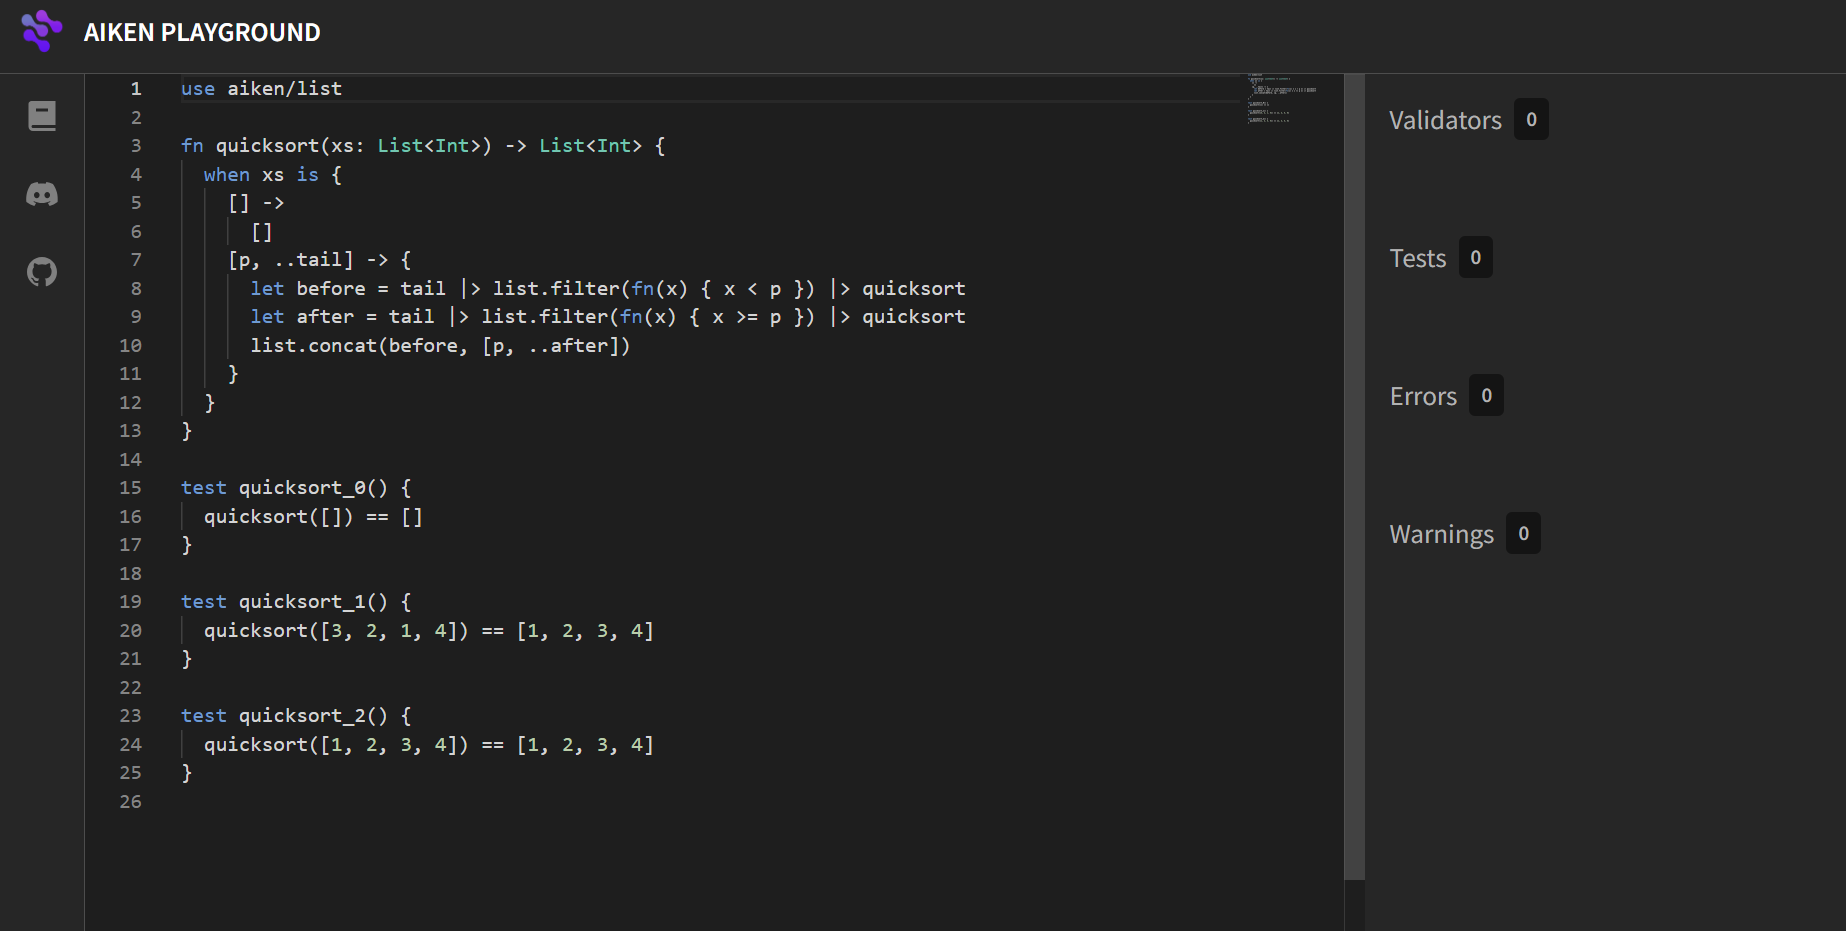
\includegraphics[scale=0.3]{aiken.png}

The Aiken Playground (\url{https://play.aiken-lang.org/}) is an online environment where developers can test and experiment with Aiken functions and smart contracts without needing to download and install the software on their local device. Similar to the Helios playground, this tool provides an easy and accessible way to get started with Aiken, allowing users to write, compile, and run Aiken code directly in the browser. It is especially useful for learning and prototyping, providing a convenient platform for exploring Aiken's features and capabilities.


\subsection{Example of a Smart Contract with Aiken}

In Aiken, we need to manually define the import libraries at the very beginning of the contract. Then, similar to Helios, we define the \texttt{Redeemer} and \texttt{Datum} types. The following smart contract will unlock the UTXO if the signer is the owner and the redeemer is the right user.

\begin{lstlisting}[language=Haskell]
use aiken/hash.{Blake2b_224, Hash}
use aiken/list
use aiken/transaction.{ScriptContext}
use aiken/transaction/credential.{VerificationKey}

type Datum {
  owner: Hash<Blake2b_224, VerificationKey>,
}

type Redeemer {
  msg: ByteArray,
}

validator {
  fn hello_world(datum: Datum, redeemer: Redeemer, context: ScriptContext) -> Bool {
    let must_say_hello =
      redeemer.msg == "Hello, World!"

    let must_be_signed =
      list.has(context.transaction.extra_signatories, datum.owner)

    must_say_hello && must_be_signed
  }
}
\end{lstlisting}


\section{OpShin Language: Concepts and Usage} \label{sec:Languages}

Opshin is an implementation of smart contracts for Cardano which are written in a strict subset of valid Python. The general philosophy of this project is to write a compiler that ensures the following:

\begin{itemize}
  \item If the program compiles, then:
  \begin{itemize}
    \item It is a valid Python program.
    \item The output running it with Python is the same as running it on-chain.
  \end{itemize}
\end{itemize}

\subsection{Why Opshin?}
\begin{itemize}
  \item \textbf{100\% valid Python:} Leverage the existing tool stack for Python, including syntax highlighting, linting, debugging, unit-testing, property-based testing, and verification.
  \item \textbf{Intuitive:} Just like Python.
  \item \textbf{Flexible:} Imperative, functional, the way you want it.
  \item \textbf{Efficient \& Secure:} Static type inference ensures strict typing and optimized code.
\end{itemize}

Opshin is a pythonic language for writing smart contracts on the Cardano blockchain. The goal of Opshin is to reduce the barrier of entry in smart contract development on Cardano. Opshin is a strict subset of Python, meaning anyone who knows Python can get up to speed with Opshin quickly.

\subsection{Setting Up the Environment}

Check out the \href{https://book.opshin.dev/}{OpShin Book} for an introduction to this tool and detailed guidance on writing smart contracts. This section outlines the basic usage of the tool.

\subsection{Installation}
Install Python 3.8, 3.9, 3.10, or 3.11. Then run:
\begin{verbatim}
python3 -m pip install opshin
\end{verbatim}

\subsection{Example of a Smart Contract}

\subsection{Example Validator - Gift Contract}
In this simple example, we'll write a gift contract that will allow a user to create a gift UTXO that can be spent by:

\begin{enumerate}
  \item The creator cancelling the gift and spending the UTXO.
  \item The recipient claiming the gift and spending the UTXO.
\end{enumerate}

\begin{lstlisting}[language=Python, caption=Gift Contract in Opshin]
# gift.py

# The Opshin prelude contains a lot of useful types and functions 
from opshin.prelude import *

# Custom Datum
@dataclass()
class GiftDatum(PlutusData):
    # The public key hash of the gift creator.
    # Used for cancelling the gift and refunding the creator (1).
    creator_pubkeyhash: bytes

    # The public key hash of the gift recipient.
    # Used by the recipient for collecting the gift (2).
    recipient_pubkeyhash: bytes

def validator(datum: GiftDatum, redeemer: None, context: ScriptContext) -> None:
    # Check that we are indeed spending a UTxO
    assert isinstance(context.purpose, Spending), "Wrong type of script invocation"

    # Confirm the creator signed the transaction in scenario (1).
    creator_is_cancelling_gift = datum.creator_pubkeyhash in context.tx_info.signatories

    # Confirm the recipient signed the transaction in scenario (2).
    recipient_is_collecting_gift = datum.recipient_pubkeyhash in context.tx_info.signatories

    assert creator_is_cancelling_gift or recipient_is_collecting_gift, "Required signature missing"
\end{lstlisting}

This might be a bit to take in, especially the logic for checking the signatures. The most important part is to see the parameters and the return type, as well as the assert statements actually controlling the validation. For more details, refer to the \href{https://book.opshin.dev/}{OpShin Book}.

\section{Plu-ts: Understanding the basics} \label{sec:Languages}

Plu-ts is a library designed for building Cardano dApps in an efficient and developer-friendly way. It is composed of two main parts:

\begin{itemize}
    \item \textbf{plu-ts/onchain:} An eDSL (embedded Domain Specific Language) that leverages TypeScript as the host language, designed to generate efficient Smart Contracts.
    \item \textbf{plu-ts/offchain:} A set of classes and functions that allow reuse of onchain types.
\end{itemize}

\subsection{Design Principles}
Plu-ts was designed with the following goals in mind, in order of importance:

\begin{itemize}
    \item \textbf{Smart Contract efficiency}
    \item \textbf{Developer experience}
    \item \textbf{Reduced script size}
    \item \textbf{Readability}
\end{itemize}

For more information, see the \href{https://book.plu-ts.dev/}{Plu-ts Book}.

\subsection{Setting Up the Environment}


\textbf{From npm:}
\begin{verbatim}
npm install @harmoniclabs/plu-ts
\end{verbatim}

\textbf{NPM:}
NPM is the package manager used by NodeJS. You can install Node and NPM from the \href{https://nodejs.org/}{NodeJS website}.

\textbf{From source:}
\begin{verbatim}
git clone https://github.com/HarmonicLabs/plu-ts
cd plu-ts
npm run build
\end{verbatim}

\textbf{The dist Folder:}
The library is then available in the \texttt{dist} folder. You can move the directory where you need it.

\subsection{Quick Start}
First, create a new directory where to build your project:
\begin{verbatim}
mkdir my-pluts-project
cd my-pluts-project
\end{verbatim}

Then initialize your Node project with npm:
\begin{verbatim}
npm init
\end{verbatim}

Install TypeScript and the TypeScript compiler \texttt{tsc} if it is not already available globally:
\begin{verbatim}
npm install --save-dev typescript
\end{verbatim}

Finally, install Plu-ts:
\begin{verbatim}
npm install @harmoniclabs/plu-ts
\end{verbatim}

\subsection{Example of a Smart Contract}

\subsection{The Contract}
In this example, we'll write a contract that expects a \texttt{MyDatum}, a \texttt{MyRedeemer}, and finally a \texttt{PScriptContext} to validate a transaction.



\begin{lstlisting}
import { Address, bool, compile, makeValidator, PaymentCredentials, pBool, pfn, Script, ScriptType, V2 } from "@harmoniclabs/plu-ts";
import MyDatum from "./MyDatum";
import MyRedeemer from "./MyRedeemer";

export const contract = pfn([
    MyDatum.type,
    MyRedeemer.type,
    V2.PScriptContext.type
],  bool)
(( datum, redeemer, ctx ) =>
    // always succeeds
    pBool( true )
);

export const untypedValidator = makeValidator( contract );
export const compiledContract = compile( untypedValidator );
export const script = new Script(
    ScriptType.PlutusV2,
    compiledContract
);

export const scriptMainnetAddr = new Address(
    "mainnet",
    new PaymentCredentials(
        "script",
        script.hash
    )
);

export const scriptTestnetAddr = new Address(
    "testnet",
    new PaymentCredentials(
        "script",
        script.hash.clone()
    )
);

export default contract;
\end{lstlisting}

This contract expects a \texttt{MyDatum}, a \texttt{MyRedeemer}, and a \texttt{PScriptContext} to validate a transaction.

\subsubsection{Custom Datum and Redeemer}
\texttt{MyDatum} and \texttt{MyRedeemer} are types defined by us in \texttt{src/MyDatum/index.ts} and \texttt{src/MyRedeemer/index.ts} respectively.

\begin{lstlisting}
import { int, pstruct } from "@harmoniclabs/plu-ts";

// modify the Datum as you prefer
const MyDatum = pstruct({
    Num: {
        number: int
    },
    NoDatum: {}
});

export default MyDatum;
\end{lstlisting}

\begin{lstlisting}
import { pstruct } from "@harmoniclabs/plu-ts";

// modify the Redeemer as you prefer
const MyRedeemer = pstruct({
    Option1: {},
    Option2: {}
});

export default MyRedeemer;
\end{lstlisting}

\subsubsection{Entry Point}
Finally, the contract is used in \texttt{src/index.ts}, which is our entry point.

\begin{lstlisting}
import { script } from "./contract";

console.log("validator compiled successfully! 🎉\n");
console.log(
    JSON.stringify(
        script.toJson(),
        undefined,
        2
    )
);
\end{lstlisting}

This index file imports the script from \texttt{src/contract.ts} and prints it out in JSON form. In this example, we see something different; instead of writing everything in the same file, we split it into several files to increase readability.

Also, note that the current contract always returns \texttt{true} as output, therefore it will always unlock the UTXO.

For more details, refer to the \href{https://book.plu-ts.dev/}{Plu-ts Book}.

The Plu-ts contract above is divided into the following key files:
\begin{itemize}
  \item \texttt{src/contract.ts} - Contains the main validator function and the script logic.
  \item \texttt{src/MyDatum/index.ts} - Defines the data structure for the Datum.
  \item \texttt{src/MyRedeemer/index.ts} - Defines the data structure for the Redeemer.
  \item \texttt{src/index.ts} - Serves as the entry point, importing and displaying the compiled script.
\end{itemize}

This organization enhances readability and separates concerns, making it easier for developers to manage and understand the contract's different components. 

In the provided example, the contract always returns \texttt{true} as the output.
This means that the contract will always validate successfully, effectively always unlocking the UTXO. While this makes the contract straightforward, it also means that the contract does not perform any meaningful validation or logic checks. 